
\chapter{Ballet Music}
\label{balletmusic}

%\section{Scores}

\section{Impressionism and Debussy: Jeux}
\begin{itemize}
\item Listen: \url{https://www.youtube.com/watch?v=eT9ZQEZQSXs}
\item Score: \url{http://imslp.org/wiki/Jeux_%28Debussy,_Claude%29}
\item Reading: \url{http://adrian-moore.staff.shef.ac.uk/teaching/mus126/debussy_jeux_eimert.pdf}
\end{itemize}

Claude Debussy (1864-1918) brings much of what we know of impressionism in painting to the musical score. Easy to say but perhaps more difficult to define. Debussy was friends with painters such as James Whistler (1834-1903). When Whistler moved to Paris in 1855 he rented a studio in the Latin Quarter (and lived the Bohemianism so often mentioned and written about). Whistler's later work is very impressionistic and he adopted the title \textit{Nocturne} to depict the obscure.      
Debussy was also heavily influenced by writers of the time such as Paul Verlaine (1844-1896) and St\'ephane Mallarm\'e (1842-1898), both symbolist writers. Symbolism focused naturally upon symbols and as a result dislocated itself from reality. As a consequence themes revolved around spirituality and the darker parts of the imagination, easily rendered through symbols (such as ravens (read E.A.Poe)). 

Mallarm\'e's poem from 1876 \textit{Pr\'elude \`a l'apr\`es-midi d'un faune} was taken by Debussy for his orchestral prelude of the same name, composed in 1894 (see table~\ref{tab:faune}). Mallarm\'e was obsessed with the musical in words and indeed wrote a sonnet to Wagner. 

\begin{figure}[H]
\centering
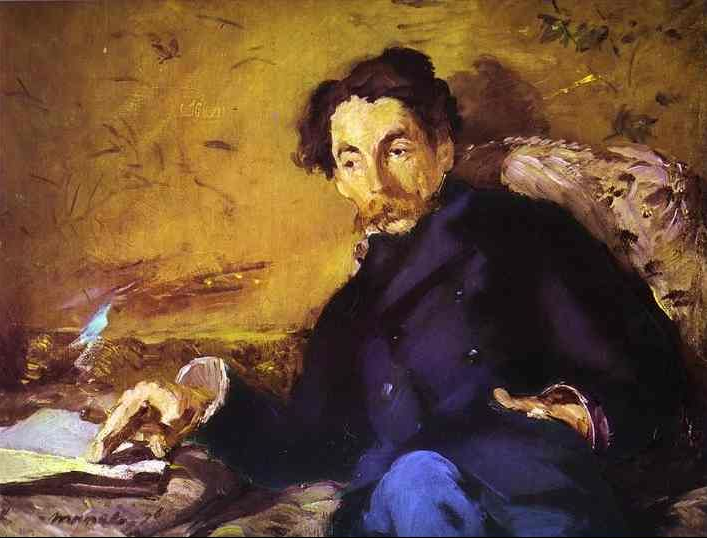
\includegraphics[scale=0.2]{manetmalarme}\caption{St\'ephane Mallarm\'e by Edouard Manet (1876)}
\label{fig:quatierlatin}
\end{figure}

\begin{table}[h!]
\begin{tabular}{|l|l|} \hline
Le Faune: & \\
Ces nymphes, je les veux perp\'etuer. & These nymphs that I would perpetuate: \\
Si clair, & so clear \\
Leur incarnat l\'eger, qu'il voltige dans l'air & And light, their carnation, that it floats in the air  \\
Assoupi de sommeils touffus. & Heavy with leafy slumbers. \\
Aimai-je un r\^eve? & Did I love a dream? \\
Mon doute, amas de nuit ancienne, s'ach\`eve & My doubt, night’s ancient hoard, pursues its theme \\
En maint rameau subtil, qui, demeur\'e les vrais & In branching labyrinths, which being still \\
Bois m\^eme, prouve, h\'elas! que bien seul je m'offrais & The veritable woods themselves, alas, reveal \\
Pour triomphe la faute id\'eale de roses. & My triumph as the ideal fault of roses. \\
R\'efl\'echissons… & Consider… \\
ou si les femmes dont tu gloses & if the women of your glosses \\
Figurent un souhait de tes sens fabuleux! & Are phantoms of your fabulous desires! \\
Faune, l'illusion s'\'echappe des yeux bleus & Faun, the illusion flees from the cold, blue eyes \\
Et froids, comme une source en pleurs, de la plus chaste: & Of the chaster nymph like a fountain gushing tears: \\
Mais, l'autre tout soupirs, dis-tu qu'elle contraste & But the other, all in sighs, you say, compares \\
Comme brise du jour chaude dans ta toison? & To a hot wind through the fleece that blows at noon? \\
Que non! par l'immobile et lasse p\^amoison & No! through the motionless and weary swoon \\
Suffoquant de chaleurs le matin frais s'il lutte, & Of stifling heat that suffocates the morning, \\
Ne murmure point d'eau que ne verse ma fl\^ute & Save from my flute, no waters murmuring \\
Au bosquet arros\'e d'accords; et le seul vent & In harmony flow out into the groves; \\
Hors des deux tuyaux prompt \`a s'exhaler avant & And the only wind on the horizon no ripple moves, \\
Qu'il disperse le son dans une pluie aride, & Exhaled from my twin pipes and swift to drain \\
C'est, \`a l'horizon pas remu\'e d'une ride & The melody in arid drifts of rain, \\
Le visible et serein souffle artificiel & Is the visible, serene and fictive air \\
De l'inspiration, qui regagne le ciel. & Of inspiration rising as if in prayer. \\

\hline
\end{tabular}
\caption{Opening of \textit{Pr\'elude \`a l'apr\`es-midi d'un faune}}
\label{tab:faune}
\end{table}

Debussy achieved success early into his student days. He entered the Paris Conservatoire in 1873 for 11 years of study. It was here that Debussy first heard Wagner's early operatic output. He continued to study with C\'esar Franck and Ernest Guiraud. He was awarded the Premier Grand Prix de Rome in 1884 for his cantata \textit{L'Enfant prodigue} (the prodigal son). Debussy was 21. You can already hear the development of phrases and the growth of romantic harmonies. But this was a hasty work, written in a month and apparently in the style of Massenet so as to please the judges of the Prix de Rome. 

As winner of the prize (which continues to this day), Debussy set off for Rome in 1885. And clearly at this time Wagner remained a huge influence (though as a master, not necessarily as one to model). Around the turn of the decade, Wagner dominated French culture, and he was particularly praised within literary circles.

Both in words and music, symbolism highlighted the sensuous. Colour took on greater significance. With the darkness of war (Franco-Prussian and ultimately WWI), artists wanted to re-inject colour into the world. But equally at that time, the Russian nationalist composers were beginning to influence European composers. The great exhibitions (such as the Paris World Fair of 1889) saw Rimsky-Korsakov conduct two concerts of Russian music. Out of this melting pot arose Debussy's early works. 

Debussy also knew Brahms and had visited and dined with him on a number of occasions. But one of his more substantial friendly relationships was with composer Erik Satie.

\subsection{Works}
Although you will probably know Debussy best by his ballet works, it is his opera \textit{Pell\'eas et M\'elisande} that should be heard more frequently. It occupied Debussy between the age of 30 and 40. \textit{Pell\'eas et M\'elisande} is a play by Maurice Maeterlink (1862-1949) written around 1893. Debussy's opera received its premiere in 1902. 

And after Nocturnes (1899) subtitled: \textit{Nuages} (clouds), \textit{F\^etes} (Festivals) and \textit{Sir\'enes} (Sirens) Debussy naturally turned to the sea with \textit{La Mer} (1903-05). We know of Debussy's intent through letters to his publisher Auguste Durand. Debussy's personal life was one of turmoil at the time too. He left his first wife, Lily, who shot herself in the heart (and survived) and took up with one Mme Emma Barda, the wife of a wealthy banker. 

Although Debussy's orchestral colour is unsurpassed, to understand his musical syntax one must go to the piano pieces. These are extraordinarily difficult to play but Debussy wrote pieces of varying technical difficulty and the `Children's Corner' pieces are excellent works to study. The first volume of \textit{Images pour piano} (1904-05) deliver that archetypal impressionistic sound that one might imagine when looking at the works of Monet (for example \textit{The Water-Lily Pond} of 1899). And indeed Debussy's works  are laced with titles such as \textit{Reflets dans l'eau}. The second set of \href{http://petrucci.mus.auth.gr/imglnks/usimg/4/4a/IMSLP254485-PMLP02391-Debussy__Claude-Images_2e_Serie_pour_Piano_seul_Durand_6994_scan.pdf}{\textit{Images}} is more complex, and is set over three staves. \textit{Cloches \`a travers les feuilles} (Bells through the leaves) uses the whole-tone scale. Other movements were titled \textit{Et la lune descend sur le temple qui fut} (And the moon descends on the temple that was), and \textit{Poissons d'or} (Golden fish). 

But it is the later works where Debussy is really experimental. The second set of Pr\`eludes becomes ever more dissonant. And in Debussy's orchestral ballet masterpiece, \textit{Jeux} (1912) we hear very detailed construction. 

\subsection{Ballets Russes and Sergei Diaghilev}
This was a time of great impresarios (Sergei Diaghilev 1872 - 1929), great choreographers (Michel Fokine 1880-1942) and even greater ballet dancers (Vaslav Nijinsky 1889 - 1950). It was clear that around 1910, ballet's maestros were no less self-absorbed. Stravinsky and Debussy were often misunderstood by Fokine and Benois (designer) who were much more involved with the day-to-day running of the company (a company which worked and toured extremely hard). 

The first dress rehearsals for \textit{Jeux} were agonising. Costumes designed by L\'eon Bakst were inappropriate and Diaghilev altered them himself. But Diaghilev was working on \textit{Jeux} and \textit{The Rite of Spring} at the same time. Jeux's opening night was 15th May 1913. The ballet is your typical `fumble in the dark' - or as outlined to the audience at the premiere:

\begin{quotation}
The scene is a garden at dusk; a tennis ball has been lost; a boy and two girls are searching for it. The artificial light of the large electric lamps shedding fantastic rays about them suggests the idea of childish games: they play hide and seek, they try to catch one another, they quarrel, they sulk without cause. The night is warm, the sky is bathed in pale light; they embrace. But the spell is broken by another tennis ball thrown in mischievously by an unknown hand. Surprised and alarmed, the boy and girls disappear into the nocturnal depths of the garden.
\end{quotation}

Nijinsky was disheartened at the reaction to \textit{Jeux} which was not riotous but lacklustre. Debussy, writing to a friend shortly after the premiere was dismayed at Nijinsky's approach which bordered (negatively) on the Dalcrozian (eurhythmics - an approach to music through movement and a form that seemingly resulted in dance that was quite leaden). 

%%continue with ballet stuff and the rite
%%emphasise the importance of the Eimert text

\subsection{The Eimert text}
The Eimert text was written in 1957 in a small but incredibly important German publication called `Die Reihe'. Eimert focuses first upon the originality of Debussy's score. Debussy clearly wrote pure music but also a number of pieces that were collaborative and \textit{Jeux} is no exception. Perhaps a quick comparison to the music for D'Annunzio's mystery play \textit{Le martyre de saint S\`bastien} might shed light upon \textit{Jeux's} originality. The music from 1911 is wholeheartedly romantic in nature. \textit{Jeux} then, might easily be heard as Debussy trying again to free his technical palette. Moreover, we should be careful not to pigeon hole \textit{Jeux} as impressionist (symbolist perhaps?). Debussy himself said of \textit{Images} and Eimert makes a point of suggesting this is even truer of \textit{Jeux}: `I am trying to introduce something new - realities, so to speak. What idiots call ``impressionism'''. Eimert proceeds to make an astute rendering of the musical score, highlighting Debussy's never-ending inventiveness.  

\subsection{Jeux: analysis starter}
The work can be easily broken down into cells and subsequent extensions. Eimert's thesis is that there is an underlying shape to the different cells. Clearly the themes are chromatic in nature and a mix of rising and falling patterns. 

\begin{figure}[H]
\centering
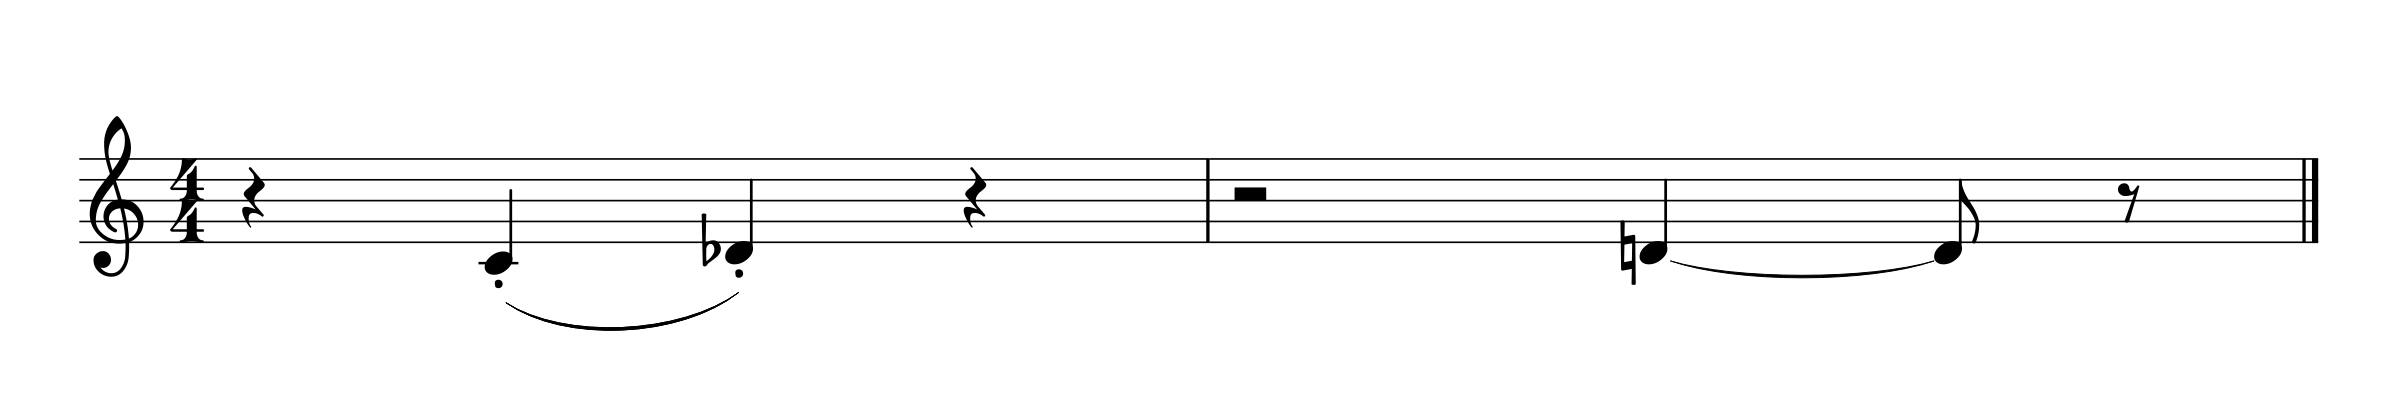
\includegraphics[scale=0.2]{jeux-cell1-1}\caption{Jeux cell1}
\label{fig:jeux1}
\end{figure}

\begin{figure}[H]
\centering
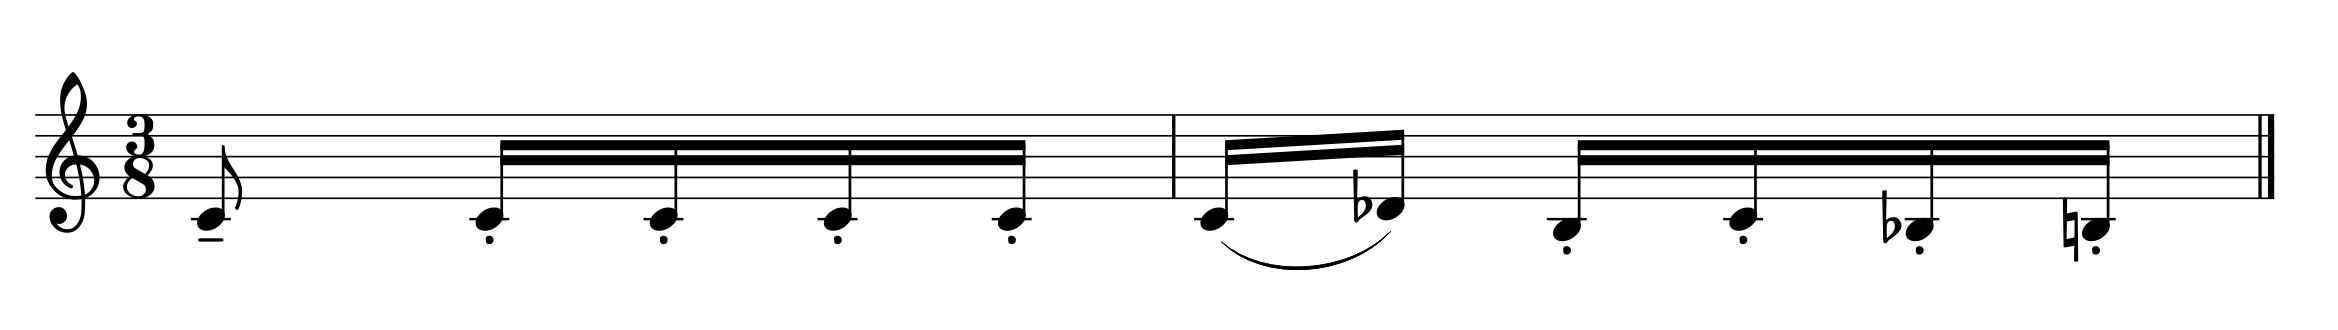
\includegraphics[scale=0.2]{jeux-cell2-1}\caption{Jeux rhythmic theme}
\label{fig:jeux2}
\end{figure}

Quite often a rise will be immediately followed by a fall, suggesting an easy ebb and flow.

\begin{figure}[H]
\centering
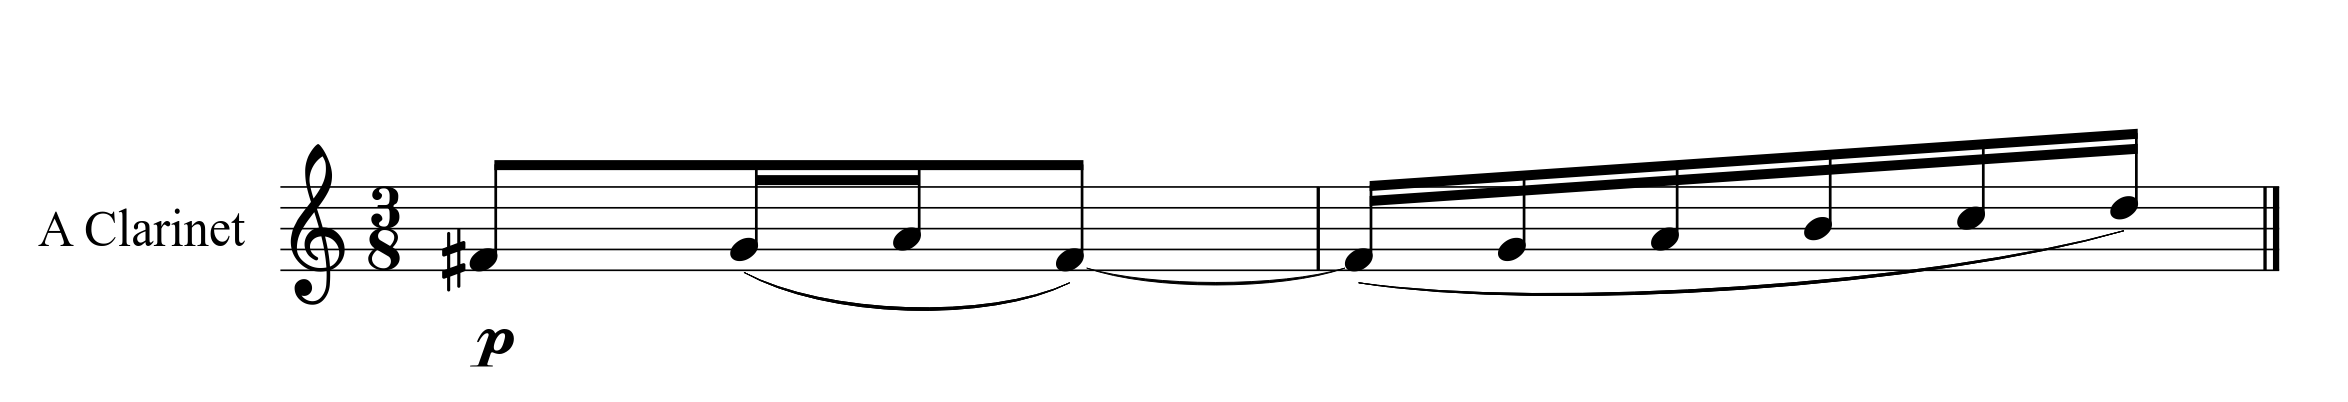
\includegraphics[scale=0.2]{jeux-cell3-1}\caption{Jeux lyric theme}
\label{fig:jeux3}
\end{figure}

Figure~\ref{fig:jeux4} is used to relax the pace and is often coloured by trills or tremolando (strings).

\begin{figure}[H]
\centering
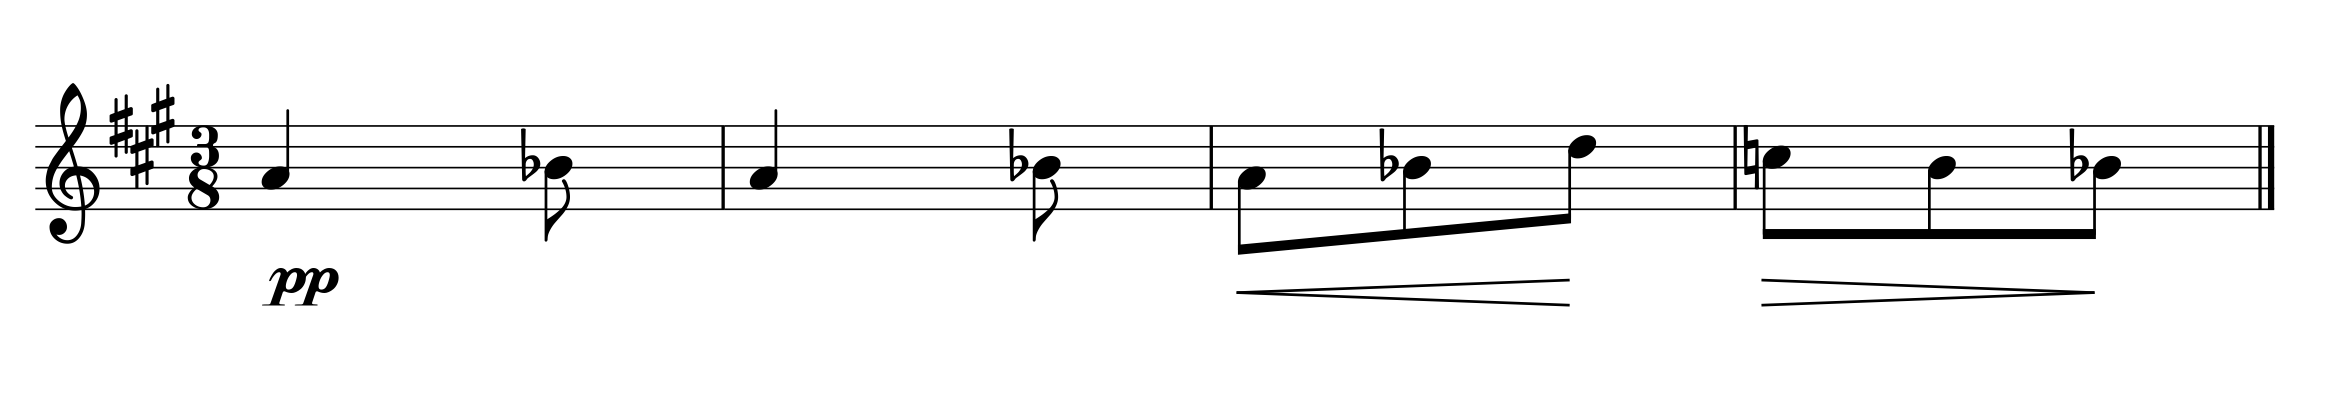
\includegraphics[scale=0.2]{jeux-cell4-1}\caption{Jeux static theme}
\label{fig:jeux4}
\end{figure}

Notice too the simple trick of inverting the theme at figure 22. 

\begin{figure}[H]
\centering
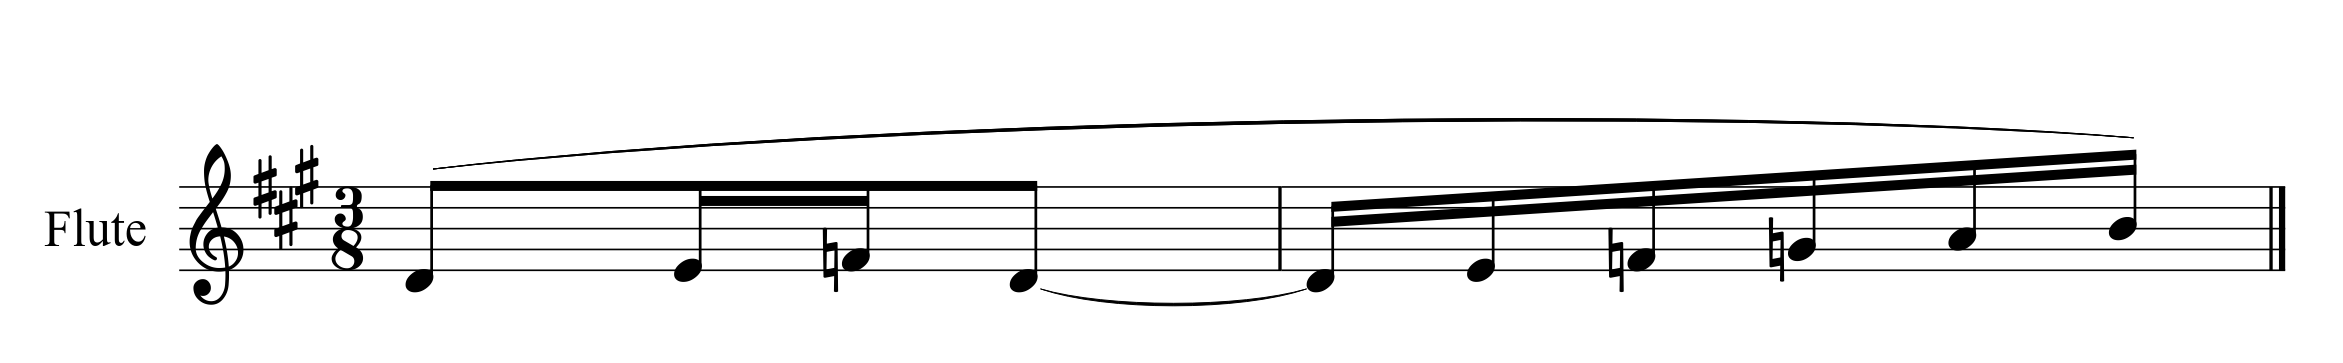
\includegraphics[scale=0.2]{jeuxfig22-1}\caption{Jeux theme inversion}
\label{fig:jeuxthemeinvert}
\end{figure}

The predominance of four bar themes (comprising 2+2) is strong. Here is the opening of section V with parallel motion oboes. Again, note the rise and fall and the dance-like `swish' at the pivot. 

\begin{figure}[H]
\centering
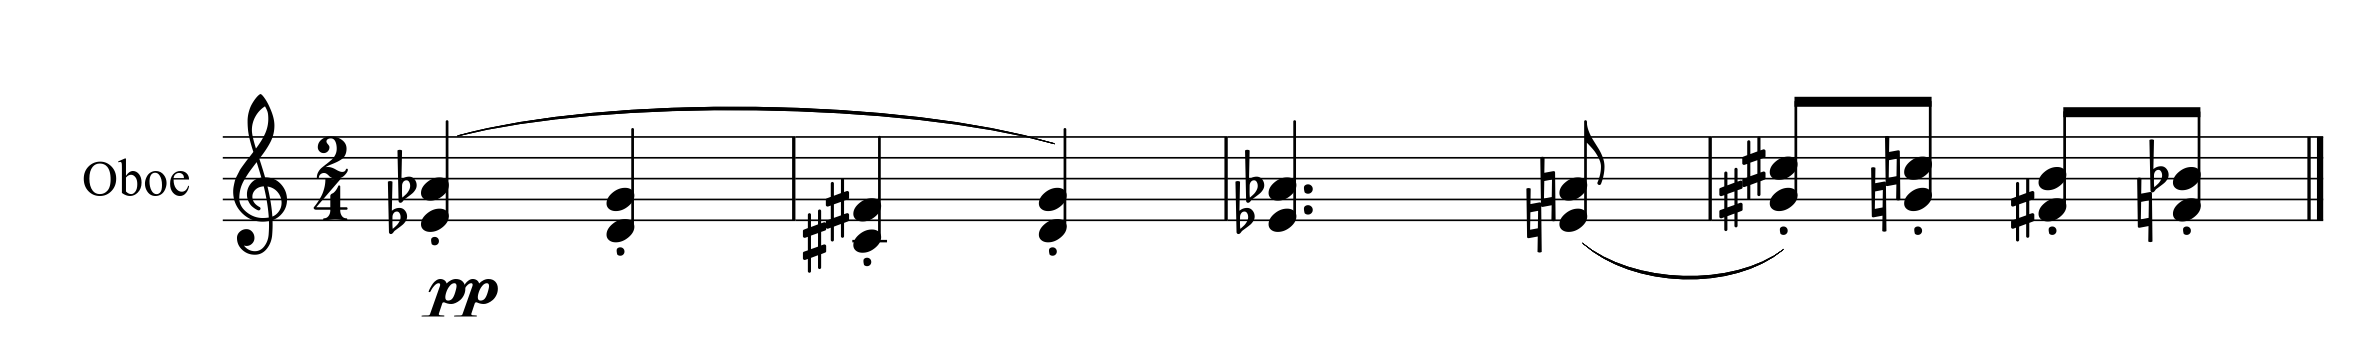
\includegraphics[scale=0.2]{jeux-section5-1}\caption{Jeux just before figure 36}
\label{fig:jeuxoboe}
\end{figure}

Notice how, at figure 38 and still in 3/8 Debussy manages to create the waltz. (Instead of the third beat being tied, it is now strongly articulated).    

As the work reaches the climax, note how the cells firm up to form ostinati reminiscent of Stravinsky's work of the same year. 

Finally, note the retrograde close (of the very first cell) to a quaint cadential `flick'. 


\section{The power of the new}
\begin{itemize}
\item \href{http://www.nytimes.com/2012/09/19/arts/music/radical-music-sometimes-shocking-sometimes-subtle.html?pagewanted=all&_r=0}{NY Times article}
\end{itemize}

\section{Modernism and Stravinsky: The Rite of Spring}
\begin{itemize}
\item Listen: \url{https://www.youtube.com/watch?v=rq1q6u3mLSM}
\item Listen: \url{https://www.youtube.com/watch?v=ewOBXph0hP4}
\item Score: \url{http://imslp.org/wiki/The_Rite_of_Spring_%28Stravinsky,_Igor%29}
\item Reading: Hill, P. (2000). Stravinsky: \textit{The Rite of Spring.} Cambridge Music Handbooks. Cambridge University Press
\item Online: \href{http://publishing.cdlib.org/ucpressebooks/view?docId=ft967nb647;brand=ucpress}{Stravinsky and the Rite of Spring: The Beginnings of a Musical Language, Pieter C. van den Toorn. 1987. University of California Press}

\end{itemize}

\begin{figure}[H]
\centering
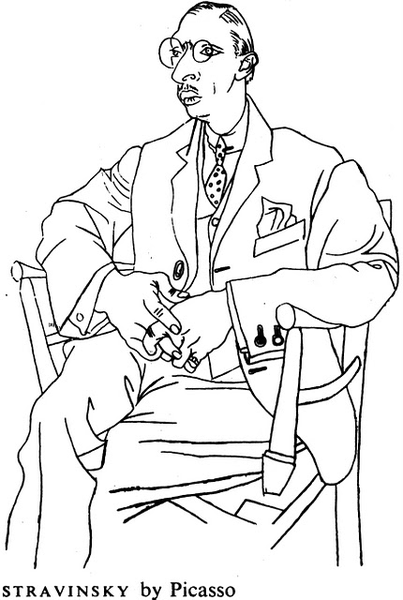
\includegraphics[scale=0.2]{Stravinsky_picasso}\caption{Stravinsky by Picasso}
\label{fig:stravpicasso}
\end{figure}

We have this account of Debussy and Stravinsky playing the four-hand piano version of the \textit{Rite}. Indeed the piano duet version of the \textit{Rite} was published in 1913, the year of the premiere; the full orchestral score was not published until 1921. The advantage of the piano version is that the orchestra is removed. The score is naked and we can hear all the dissonance and rhythmic complexity. 

Stravinsky's first collaboration with Diaghilev was \textit{The Firebird}. Diaghilev's original choice of composer was Liadov (Diaghilev's old harmony tutor) and when he showed no interest Diaghilev turned to the pupil of Rimsky-Korsakov, who was Stravinsky. There is a moment when, in December 1909 Diaghilev telephones Stravinsky to offer him the commission and Stravinsky attests to having already begun the work such is Stravinsky's assuredness. 

Diaghilev was inspried by Wagner's total control over the artwork but was less interested in the financial outlay required to stage opera so focused upon ballet. After \textit{Firebird} came \textit{Petrushka} in 1911. (Diaghilev had had great success with a ballet set to Rimsky-Korsakov's \textit{Sch\'eh\'erazade} and was clearly a proponent of new music). Stravinsky was paid 1500 roubles for \textit{The Firebird} and due to its success, he knew there would be further opportunities. And it was at this point that Stravinsky began to think about the \textit{Rite}. As he wrote to the painter Roerich:

\begin{quotation}
Naturally, the success of \textit{The Firebird} has encouraged Diaghilev for future projects, and sooner or later we will have to tell him about the `Great Sacrifice'....As soon as I said that I was working with you, both Diaghilev and Bakst were delighted, Bakst saying he thought our idea was a noble one. They were greatly relieved, obviously, to hear that my secret did not concern Benois: Diaghilev would have been greatly offended if Benois had been involved. \citep[p176]{buckle1975diaghilev}
\end{quotation}

In the Summer of 1910, Diaghilev and Nijinsky arrived at Stravinsky's studio and instead of hearing early work on the \textit{Rite} got a new composition: \textit{Petrushka} - Petrushka being a Russian version of the Punch story. 

We should also remember that Ravel, the great orchestrator had been commissioned by Diaghilev in 1908 to write \textit{Daphnis et Chlo\'e} a ballet of huge proportions. Diaghilev was, at this time almost bankrupt but was still commissioning work. 

It was Diaghilev's aspiration for greatness that led to this outpouring of new music. By 1910 he was looking to form his own company and was waiting for the time when Nijinsky would begin to choreograph his own movement. (Until this time Fokine was doing this). But Nijinsky began to take control as he sketched steps to Debussy's \textit{L'Apre\`es-midi d'un faune}. As Stravinsky wrote to his mother in April 1912:

\begin{quotation}
Diaghilev and Nijinsky are mad about my new child, \textit{Le Sacre du printemps.} The unpleasant part is that it will have to be done by Fokine whom I consider an exhausted artist, one who has travelled his road quickly and who writes himself out with each new work. \textit{Sch\'eh\'erazade} was the high point of his achievement and, consequently, the beginning of his decline. \citep[p219]{buckle1975diaghilev}
\end{quotation}

Fokine left the company in June 1912 and Nijinsky danced \textit{La Sacre du printemps} at the Th\`e\^atre des Champs-\'Elys\'ees on 29 May 1913. Diaghilev, ever the conjourer of spetacle had given free tickets to young artists and fans. Thus was the melting pot set: the rich and famous seated in their boxes; the unruly standing up. The riot is well documented. Diaghilev had the house lights turned up at the change of scene and the police were called in to remove the most unruly. Both Ravel and Delius were present at the premiere. The ballet company continued apace, the music set its place in history. 

\begin{figure}[H]
\centering
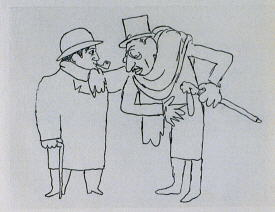
\includegraphics[scale=1.0]{picassostrav_cocteau}\caption{Stravinsky and Picasso by Jean Cocteau}
\label{fig:stravpicasso_cocteau}
\end{figure}

Stravinsky went on to write \textit{Les Noces}, \textit{Pulcinella} and \textit{Apollo} during a composing career of over 60 years.  

Peter Hill's key text \citeyearpar{hill2000stravinsky} accounts for some of the folk music `borrowings'. The opening bassoon line was the only tune Stravinsky acknowledged to be of folk origins. The odd lyrical theme contrasts against the new and brutal harmony. Triads are superposed as in figure~\ref{fig:augurschord} 

\begin{figure}[H]
\centering
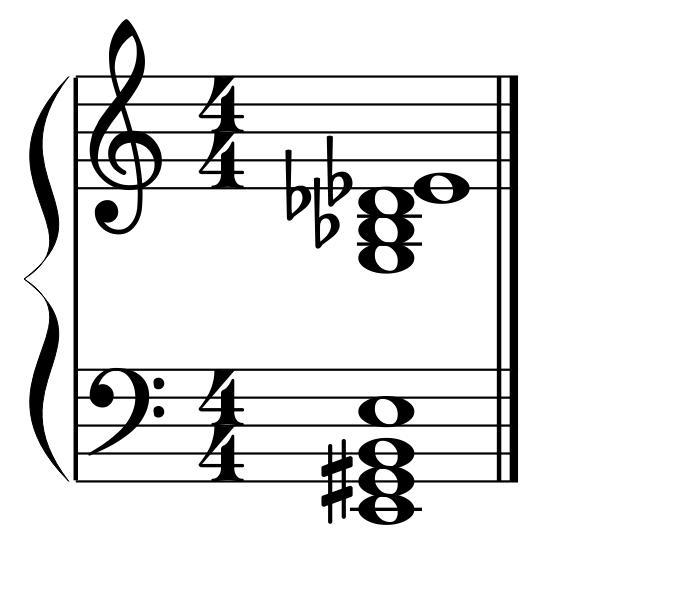
\includegraphics[scale=0.15]{augurschord}\caption{Augurs of Spring}
\label{fig:augurschord}
\end{figure}

The octotonic scale is used (see pages 44 and on in Hill). Hill talks about minor tetrachords (a four note combination) that is the first four notes of a minor scale (Tone, Semi-tone, Tone). Note this use in Ritual of the Rival Tribes.

\begin{figure}[H]
\centering
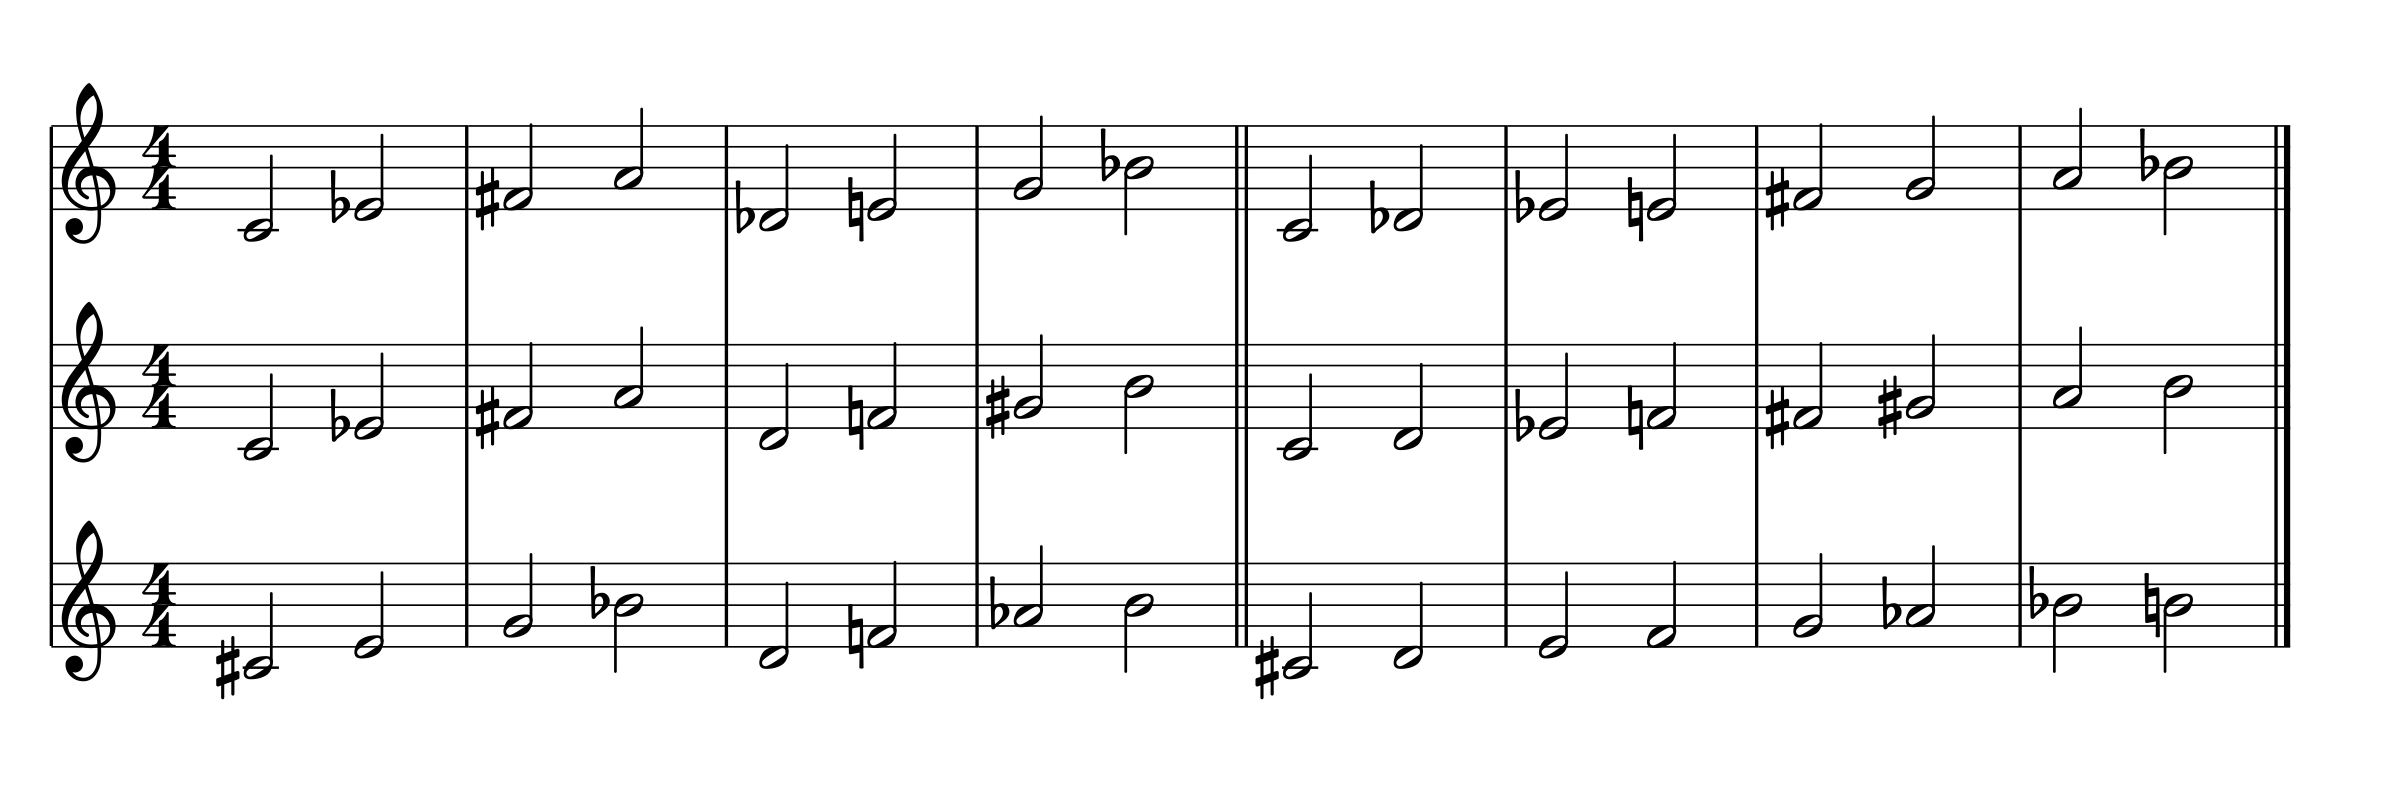
\includegraphics[scale=0.2]{octophonics}\caption{Ocotphonic collections}
\label{fig:octophonics}
\end{figure}

\begin{figure}[H]
\centering
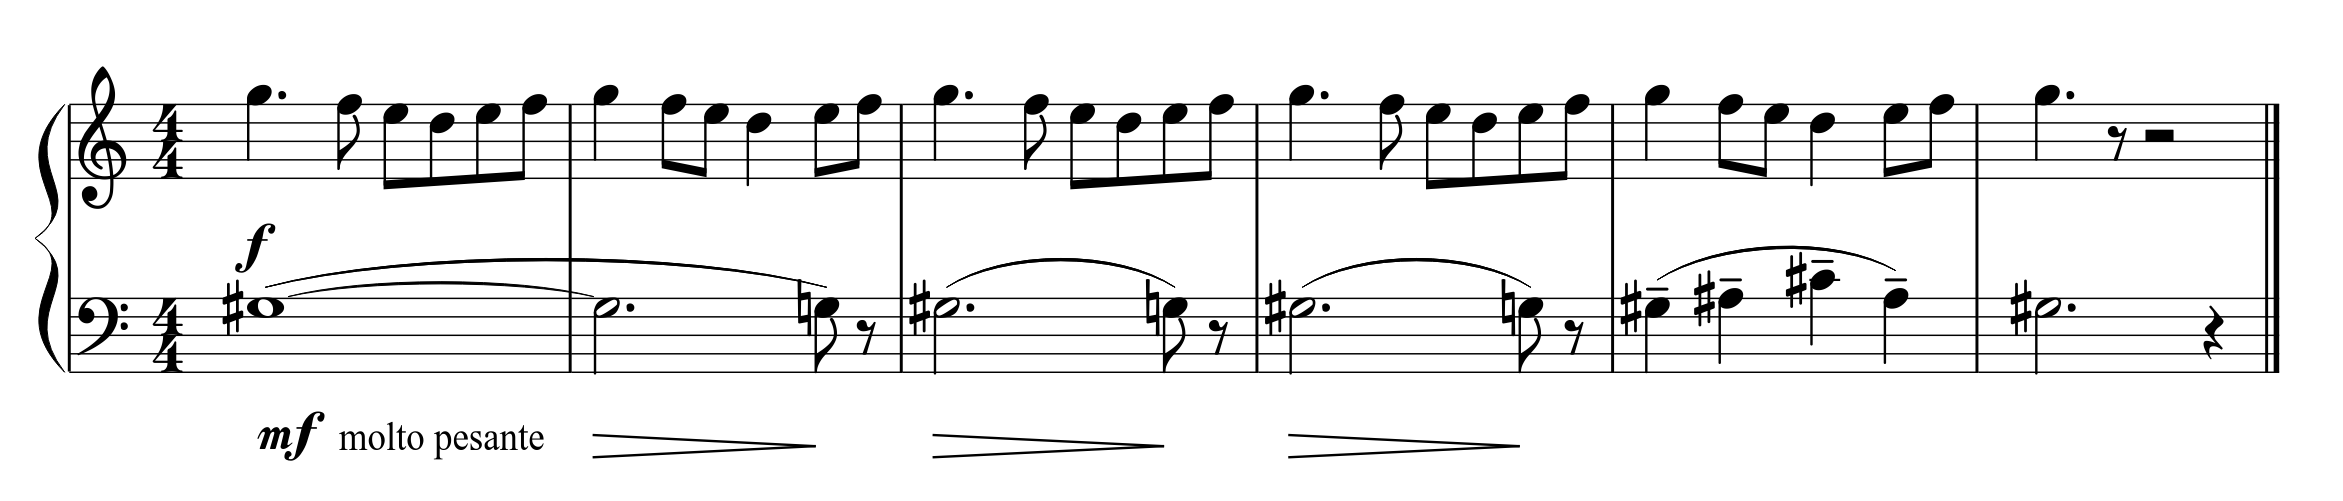
\includegraphics[scale=0.2]{rivaltribes}\caption{Ritual of the Rival Tribes}
\label{fig:rivaltribes}
\end{figure}

Note also the use of superposed intervals. 

\begin{figure}[H]
\centering
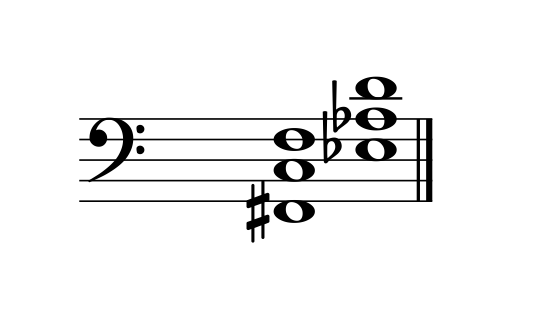
\includegraphics[scale=0.2]{fourthschord}\caption{The fourths chord at the 11/4 before Glorification}
\label{fig:fourthschord}
\end{figure}

\subsection{Rhythm: Sacrificial Dance}

It is hard not to imagine anything else so ritualistic as the rhythmic drive of the Sacrificial Dance, a framework for equally brutal chord clusters. 

\begin{figure}[H]
\centering
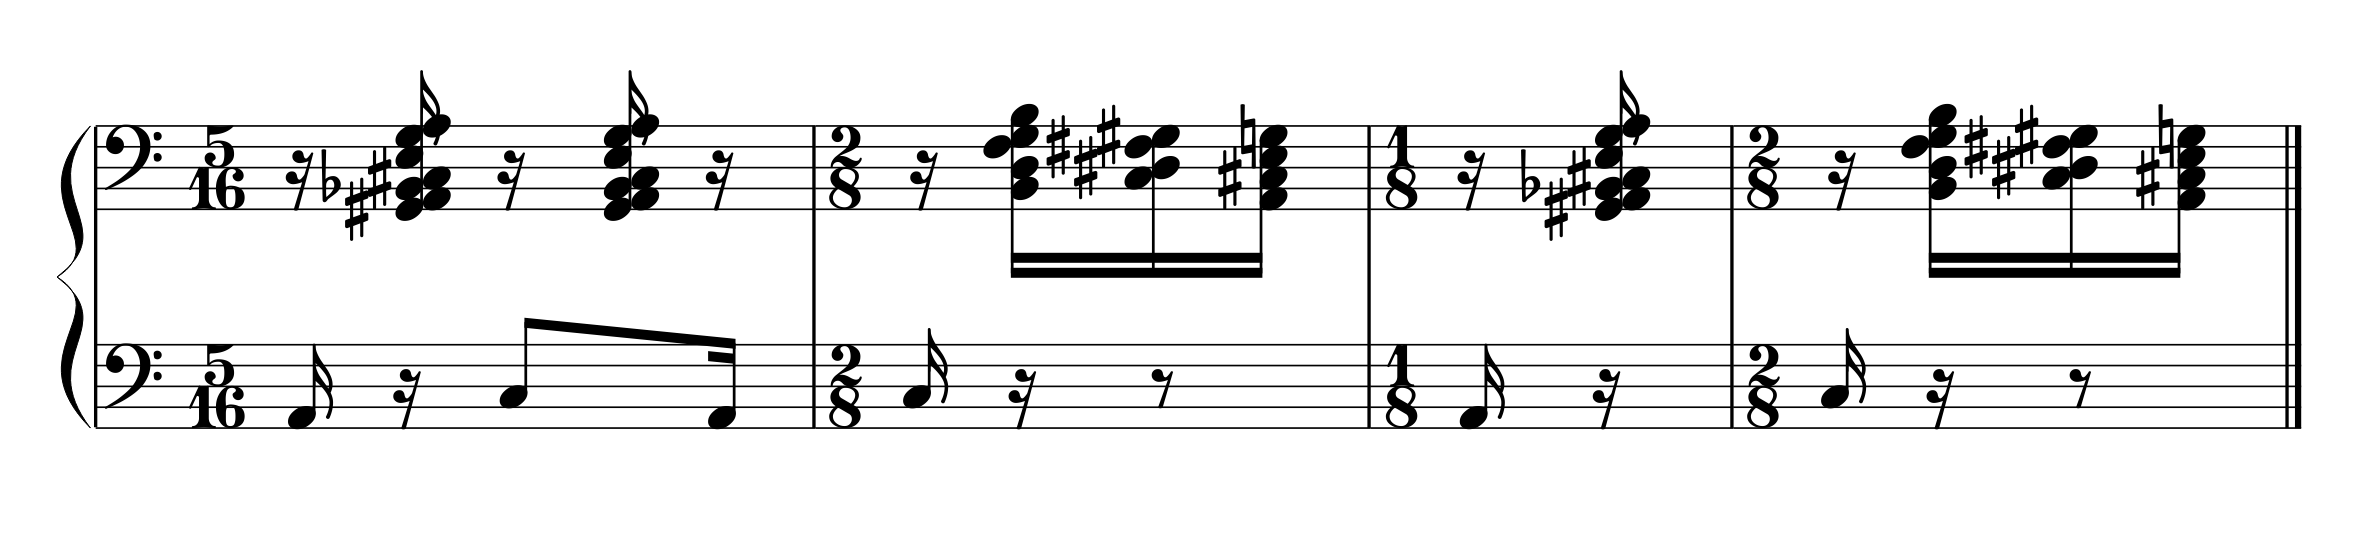
\includegraphics[scale=0.2]{sacrificialdance1}\caption{Sacrificial Dance}
\label{fig:sacrificialdance1}
\end{figure}

\begin{figure}[H]
\centering
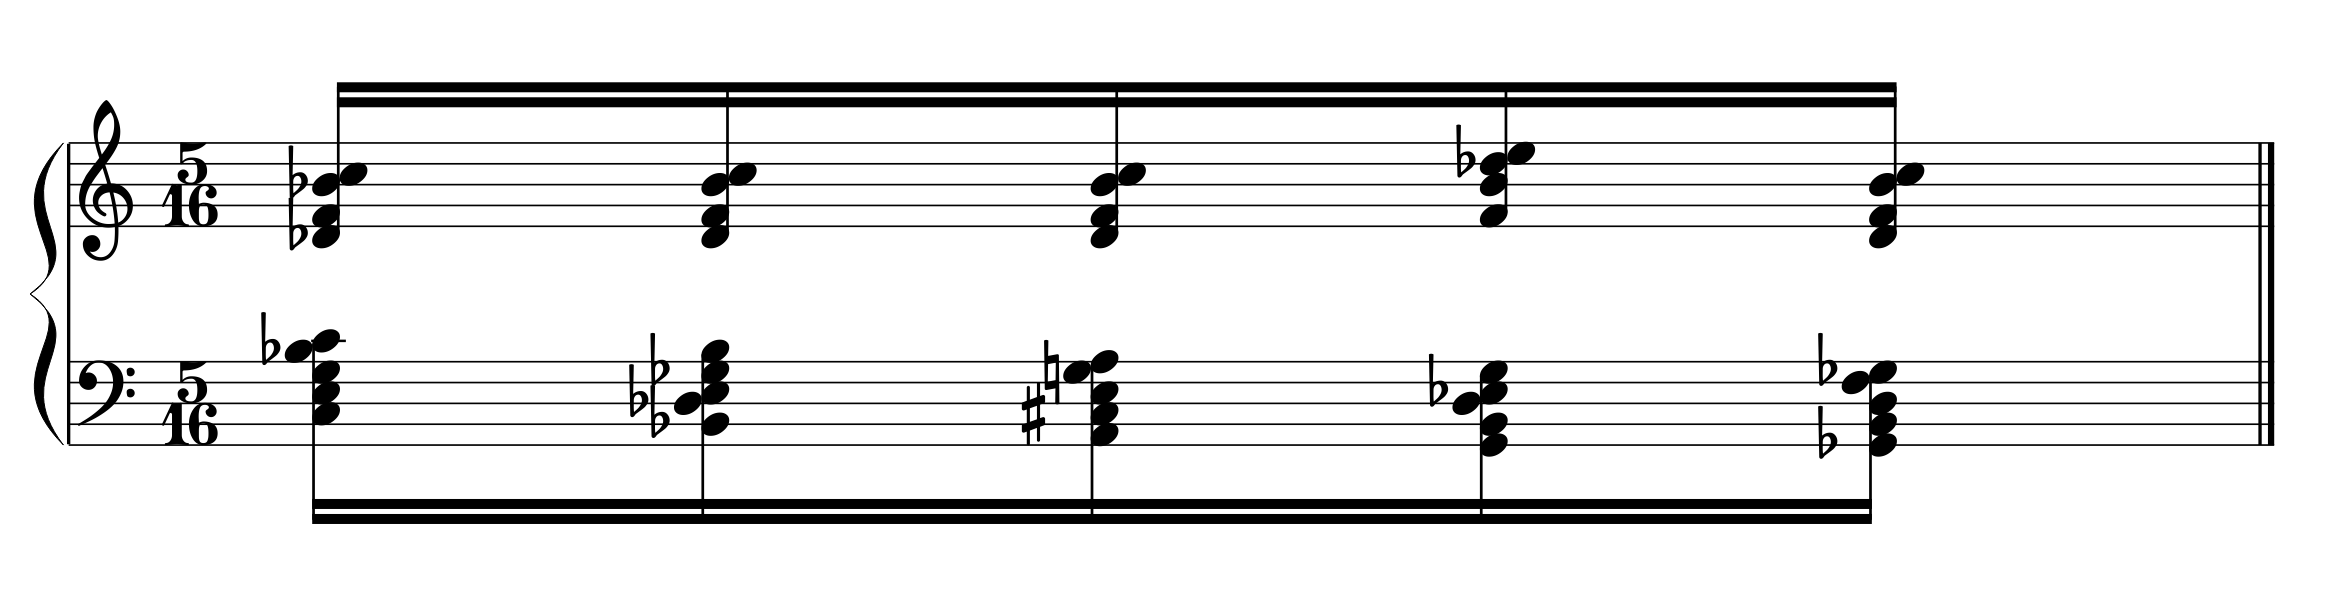
\includegraphics[scale=0.2]{sacrificialdance2}\caption{Interruption 5/16}
\label{fig:sacrificialdance2}
\end{figure}

It will be worth commenting upon the music's main moments - in particular the use of ostinato in various numbers and the continuing development of rhythm. Having listened to the piano version it will also be useful to look at orchestration. 




